\chapter{Encoding and Decoding}
\label{ch:encoding-decoding}

Four bytes lie in memory at the program counter. They are values until a
decoder treats them as an instruction. The decoder may produce an operation
and operands, reject the pattern, or consume a different number of bytes than
a neighboring architecture would. None of those choices yet says what the
decoded instruction does.

This boundary is where software becomes unusually literal. A compiler may
intend an addition. An assembler may print an addition. A disassembler may
report an addition. The processor receives bytes. If the route from those
bytes to the intended instruction is wrong, every later proof begins with the
wrong object.

\begin{keyidea}[title={Bytes, instructions, and effects are different objects}]
An encoding is a byte string. Decoding maps that string, in a declared mode,
to an instruction instance or a rejection. Execution maps the instruction
instance and a state to a successor state. Assembly is notation for humans.
Evidence about one map does not automatically establish the other.
\end{keyidea}

\section{Why instruction encodings exist}

An early stored-program machine needed a way to place operations and their
arguments in the same finite storage used for numbers. That choice made a
program inspectable, movable, and mechanically fetchable. It also created a
permanent design problem: which parts of a finite word name the operation,
which parts name operands, and what happens to patterns that have no assigned
meaning?

A regular format gives the decoder fixed places to look. It can make hardware,
teaching, and formalization easier. It may spend bits on fields an instruction
does not need. A variable format can give common instructions short spellings
and retain compatibility with older ones. It makes the first question---how
many bytes belong to this instruction?---part of decoding itself.

Neither choice is simply ``modern'' or ``old.'' RISC-V's base integer format
uses regular 32-bit instructions, while its optional compressed extension adds
16-bit forms. x86-64 retains a variable-length family shaped by decades of
compatible extension. The useful comparison is not a slogan about RISC and
CISC. It is a list of exact decoder obligations.

\begin{archive}[title={Compatibility leaves marks in the byte stream}]
Instruction formats are historical records. A field may exist because an
earlier machine needed it. A prefix may acquire a new role in a later mode.
An opcode region may be reserved so that a future extension has somewhere to
grow. Reading an encoding is therefore partly mathematics and partly careful
historical interpretation of a versioned specification.
\end{archive}

The rest of this chapter uses one addition on three machines. A0 makes every
field visible. RV64I shows a regular commercial-scale design. x86-64 shows a
short variable-length instruction whose meaning depends on a prefix and an
operand byte. The arithmetic result is familiar. The path used to select that
arithmetic is not.

\section{Four objects, not one}

We will keep four representations separate.

\begin{description}
\item[Assembly spelling.] Text such as \code{add r3, r5, r2}. It depends on a
syntax and may contain aliases.
\item[Instruction bytes.] A finite sequence such as \code{10 2B 02 00}. Byte
order and length are explicit.
\item[Decoded instance.] A structured value such as
\(
  \mathrm{Add}(rd=3,rs1=5,rs2=2).
\)
\item[Transition rule.] The rule that reads two registers, writes their
fixed-width sum, updates declared conditions, advances the program counter,
and preserves everything else.
\end{description}

An assembler normally maps spelling to bytes. A decoder maps bytes to an
instance. A disassembler maps an instance or bytes back to a chosen spelling.
The reverse maps need not recover the original text because several spellings
can denote the same instruction. A proof should therefore use the structured
instance as its semantic hinge rather than requiring printed text to round
trip character for character.

\begin{warning}[title={A successful disassembly is not an execution proof}]
A disassembler can correctly identify an instruction while an executor gives
that instruction the wrong effect. An executor can implement addition
correctly while its decoder assigns addition to the wrong byte pattern. Test
and prove the two maps separately before testing their composition.
\end{warning}

The mode belongs to the decoder input. The same x86 byte sequence can be
interpreted differently in different execution modes. The enabled RISC-V
extensions determine whether some patterns are ordinary instructions,
compressed instructions, hints, reserved encodings, or illegal encodings. A
decoder whose type is merely \(
\textit{bytes}\to\textit{instruction}
\) hides information needed to state its contract.

A more honest decoder accepts a source pin, mode, feature set, address, and
byte sequence. Its result has the shape
\[
  \mathrm{Decoded}(i,n)\quad\hbox{or}\quad\mathrm{Reject}(r),
\]
where \(n\) is the number of bytes consumed and \(r\) is a declared rejection
reason. A0 fixes most of these parameters, but keeping the full shape in view
prevents the small model from teaching an accidental universal rule.

\subsection{A decoder is total when rejection is a result}

A useful decoder function returns an answer for every finite input supplied to
its declared interface. That answer need not be an instruction. It may say
that the bytes are incomplete, the address is misaligned, the pattern is
reserved, the requested feature is disabled, or the form lies outside the
implemented slice. Making these cases explicit avoids host-language exceptions
and silent fallbacks becoming accidental architecture semantics.

\begin{figure}[htbp]
\centering
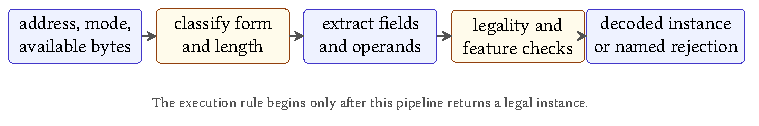
\includegraphics[width=0.98\textwidth]{figures/decoder-stage-pipeline}
\caption{A staged decoder returns either a structured instruction or a named
rejection. Execution begins only after decoding succeeds.}
\figalt{Address mode and bytes pass through form and length classification, field extraction, legality checks, and finally a decoded instance or rejection.}
\label{fig:decoder-stage-pipeline}
\end{figure}

Incomplete input differs from an illegal complete encoding. A fixed-four-byte
decoder given only three available bytes cannot yet inspect all reserved
fields. A streaming decoder may request another byte. A fetch model may trap
because the fourth address is unreadable. By contrast, four available A0 bytes
with a set reserved bit form a complete pattern that the legality rule rejects.
The surrounding step semantics decides how each decoder result becomes a
machine outcome.

Address belongs in the input even for fixed-length formats. A0 and the selected
RV64I subset require aligned instruction addresses. For variable-length x86,
the address also determines which byte begins the parse. Starting one byte
later can produce a different legal instruction sequence from the same memory.
A decoder over an isolated byte array should therefore state that element zero
is already the chosen instruction boundary.

\begin{definition}[title={Decoder result and fetch result}]
A decoder result classifies supplied bytes under a mode and feature set. A
fetch result determines which bytes are available from machine memory at a
program counter and whether reading them is permitted. Keeping the two
relations separate allows the same pure decoder to be tested without claiming
that every supplied byte string is fetchable in a running machine.
\end{definition}

This separation also improves controls. Truncating the buffer should exercise
an incomplete-input path. Setting a reserved bit should exercise legality.
Changing the start address should exercise alignment or boundary selection.
One generic rejection loses the evidence that all three checks actually fire.

\section{A0: every byte has a job}

Every A0 instruction occupies four bytes and begins at an address divisible
by four. The program map is read in increasing address order.

\begin{figure}[htbp]
\centering
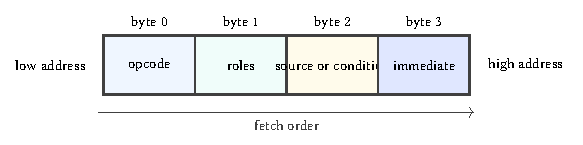
\includegraphics[width=0.84\textwidth]{figures/a0-encoding}
\caption{The four-byte A0 envelope. The detailed meaning of bytes 1--3 depends
on the opcode, but their locations and the total length never change.}
\figalt{Four boxes in fetch order labeled opcode, roles, source or condition, and immediate.}
\label{fig:a0-encoding}
\end{figure}

Byte 0 is the opcode. In byte 1, bits 0--2 name \(rd\), bits 3--5 name
\(rs1\), and bits 6--7 are reserved zero. In byte 2, bits 0--2 name
\(rs2\), bits 3--5 hold a branch condition, and bits 6--7 are reserved zero.
Byte 3 holds a signed eight-bit immediate when the instruction uses one. An
unused field must be zero. This last rule makes A0 stricter than a decoder that
merely ignores irrelevant bits.

Consider
\begin{codelisting}[language={},caption={One A0 register addition}]
add r3, r5, r2
\end{codelisting}
The opcode is \code{10}. Packing \(rd=3\) and \(rs1=5\) into byte 1 gives
\[
  3+(5\mathbin{\ll}3)=3+40=43=\mathtt{2B}.
\]
Byte 2 contains \(rs2=2\), so it is \code{02}. Addition has no immediate or
branch condition, so byte 3 and every unused field are zero. The complete
encoding is
\[
  \mathtt{10\ 2B\ 02\ 00}.
\]

The decoder performs the argument in reverse. It checks the fetch address and
length, reads opcode \code{10}, rejects any set reserved bit, extracts the
three register numbers, checks that the condition and immediate fields are
zero, and returns
\(
\mathrm{Add}(3,5,2)
\).

\begin{proofkit}[title={A0 addition round trip}]
Let \(E\) be the encoder for a legal A0 addition and \(D\) the decoder. To
show \(D(E(rd,rs1,rs2))=\mathrm{Add}(rd,rs1,rs2)\), use the fact that
each register number is below eight. Masking the packed byte by \code{07}
recovers \(rd\). Shifting it right by three and masking by \code{07} recovers
\(rs1\). The same mask recovers \(rs2\) from byte 2. The encoder writes zero
to every reserved and unused field, so all legality checks pass.
\end{proofkit}

That proof has a converse worth stating carefully. If the decoder accepts an
A0 addition byte string \(b\), encoding the returned instance reproduces
\(b\). Acceptance matters. Without it, a byte string with a reserved high bit
could decode to the same three registers after masking but fail to reproduce
the original byte. The reserved-bit check is what makes accepted encodings
canonical.

\begin{tryit}[title={Break the A0 encoding one field at a time}]
Begin with \code{10 2B 02 00}. Change byte 1 to \code{6B}, which sets a
reserved bit. Change byte 2 to \code{0A}, which leaves \(rs2=2\) but sets an
unused condition bit. Change byte 3 to \code{01}. A strict decoder rejects all
three. A decoder that only extracts operands accepts them, revealing three
different omissions in one small test family.
\end{tryit}

Illegal encodings are not gaps outside the semantics. If a running A0 state
fetches a complete but illegal instruction, its next state is trapped with an
illegal-encoding reason. Thus the decoder's rejection becomes an architectural
event through the step relation.

\subsection{Canonical encoding is stronger than successful decoding}

A decoder could ignore every unused A0 field and still recover the intended
operation and operands from encodings produced by the official encoder. Such a
decoder satisfies the forward round trip on encoder output. It fails the
canonicality contract because many byte strings with nonzero unused fields
would be accepted as the same instruction.

Canonical encodings provide one byte representation for each legal A0
instance. This makes byte equality and instruction equality coincide on
accepted inputs:
\[
  D(b_1)=D(b_2)\quad\hbox{implies}\quad b_1=b_2.
\]
The implication relies on reserved and unused field checks. It would be false
in an architecture that intentionally permits several encodings of one
instruction.

\begin{proofkit}[title={Accepted A0 encodings are injective}]
Suppose two accepted A0 byte strings decode to the same instruction instance.
The opcode and every used operand field must match that instance. Acceptance
forces all reserved and unused fields to their canonical zero values. Each
byte is therefore determined by the common instance, so the byte strings are
equal. The same argument would fail if the decoder merely masked away an
unused set bit.
\end{proofkit}

Canonicality helps evidence handling. A manifest can store the legal bytes and
the decoded object without choosing among aliases. It does not eliminate the
need to store both: the bytes bind the claim to the program image, while the
instance binds execution to structured operands. A digest of only one layer
cannot detect every substitution in the other.

Real ISAs may admit aliases at the assembly or encoding level. A
disassembler can also choose a preferred spelling that differs from the source
text. Their correct round-trip property may therefore use normalization:
decode, re-encode to a designated canonical form, and compare meanings rather
than demand reproduction of the original spelling.

\section{RV64I: one word, several fields}

The RV64I base integer ISA uses 32-bit base instructions. The optional
compressed extension can add 16-bit instructions, but we exclude that
extension in this example. The source pin is the ratified unprivileged
architecture, version 20260120; RV64I itself is version 2.1
\autocite{riscv2026unpriv}.

An R-type instruction divides the 32-bit word into six fields.

\begin{figure}[htbp]
\centering
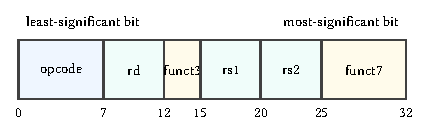
\includegraphics[width=0.96\textwidth]{figures/rv64-r-format}
\caption{The RV64I R-type format, drawn from least-significant bit at left to
most-significant bit at right. Printed manuals often reverse that direction.}
\figalt{A 32-bit bar with opcode in bits 0 to 6, rd 7 to 11, funct3 12 to 14, rs1 15 to 19, rs2 20 to 24, and funct7 25 to 31.}
\label{fig:rv64-r-format}
\end{figure}

For \code{add x3, x5, x2}, the fields are
\[
\begin{array}{c|c|c}
\mathrm{field} & \mathrm{value} & \mathrm{role}\\ \hline
\mathit{opcode} & \mathtt{0110011} & \mathrm{integer\ register\ operation}\\
\mathit{rd} & 3 & \mathrm{destination}\ x3\\
\mathit{funct3} & \mathtt{000} & \mathrm{operation\ selector}\\
\mathit{rs1} & 5 & \mathrm{first\ source}\ x5\\
\mathit{rs2} & 2 & \mathrm{second\ source}\ x2\\
\mathit{funct7} & \mathtt{0000000} & \mathrm{operation\ selector}
\end{array}
\]
Packing these fields gives the word \code{002281B3}. In little-endian memory,
the four bytes at increasing addresses are
\[
  \mathtt{B3\ 81\ 22\ 00}.
\]
The field diagram describes bit positions in the 32-bit instruction word. The
byte sequence describes memory addresses. Confusing those two views is a
common source of reversed examples.

The opcode alone does not identify \code{add}. It identifies the broad
register-operation class. The \textit{funct3} and \textit{funct7} fields
complete the selection. Changing \textit{funct7} from \code{0000000} to
\code{0100000} while leaving the other fields fixed changes this instance to
\code{sub x3, x5, x2}. Changing only \textit{funct3} can select another
operation in the same broad class.

\begin{example}[title={Decode from bytes without reading the mnemonic}]
Read \code{B3 81 22 00} as a little-endian 32-bit word. Bits 0--6 are
\code{0110011}. Bits 7--11 give 3; bits 12--14 give 0; bits 15--19 give 5;
bits 20--24 give 2; and bits 25--31 give 0. The table for the pinned RV64I
version assigns that complete field combination to \code{add x3,x5,x2}.
Only after this selection should the execution rule read \(x5\), read \(x2\),
write their modulo-\(2^{64}\) sum to \(x3\), and advance the program counter.
\end{example}

RV64I adds another semantic condition absent from A0: register \(x0\) reads as
zero, and writes to it have no architectural effect. The encoding still has a
five-bit destination field when its value is zero. Decoding
\code{add x0,x5,x2} must retain that destination in the instruction instance;
the execution rule supplies the discard behavior. Erasing the operand during
decode would mix a state rule into a format rule.

Reserved and hint encodings require the same care. A pattern's status depends
on the exact ISA and extension set. ``My current processor does nothing
visible'' does not establish that a pattern is universally a no-operation.
The book will name the enabled subset before assigning meaning.

\subsection{Regular length does not mean one field layout}

RV64I base instructions in this window share a 32-bit length, but their fields
do not all play the same roles. R-type arithmetic has two source registers and
one destination. I-type arithmetic and loads replace the second register field
with immediate bits. Stores need two registers but no destination, so their
immediate is split around the other fields. Conditional branches also split
and rearrange a signed displacement.

The decoder must reconstruct a logical immediate before sign extension. For a
split field, concatenating pieces in memory-byte order is wrong; the source
specification assigns each instruction bit to a particular result bit. Once
the pieces are placed, the high immediate bit determines sign extension to the
architectural calculation width. Scaling or an implicit zero low bit is a
separate step for forms that require it.

\begin{example}[title={Field extraction precedes interpretation}]
Suppose a 12-bit I-type immediate field is \code{FFF}. Extraction first
returns the 12-bit pattern with value 4095 under an unsigned reading. The
instruction rule then sign-extends that pattern, producing -1 under its signed
reading and an all-ones 64-bit word. Calling the field itself negative before
naming its width and extension rule compresses two operations into one.
\end{example}

Instruction selection and operand construction are likewise distinct. The
opcode and function fields may select a load class; another field selects the
load width and extension policy; register and immediate fields construct its
operands. A decoder result should preserve those decisions explicitly so the
executor does not inspect raw instruction bits again and create a second,
possibly inconsistent decoder.

\begin{warning}[title={Do not sign-extend before reassembling a split field}]
Sign-extending each fragment separately invents high bits that were never part
of the immediate. Place every fragment into the declared logical field, then
apply the one extension rule to the complete field.
\end{warning}

The feature set remains load-bearing even at fixed length. A 32-bit pattern
reserved in RV64I may acquire meaning under an enabled extension. Soundness is
therefore relative to the declared ISA string, not merely to XLEN and the word
value. A decoder that accepts extension forms while claiming the base subset is
too permissive; one that rejects enabled forms may be sound but incomplete for
the larger scope.

\section{x86-64: length is part of the answer}

In 64-bit mode, an x86 instruction can contain legacy prefixes, a REX prefix,
an opcode, a ModR/M byte, an optional SIB byte, an optional displacement, and
an optional immediate. Not every instruction contains every part. The decoder
must decide which parts are present as it moves through the byte stream. Our
source is Intel's version 092 instruction reference
\autocite{intel2026sdm2}.

Consider Intel-syntax \code{add rax, rbx}. One encoding is
\[
  \mathtt{48\ 01\ D8}.
\]

\begin{figure}[htbp]
\centering
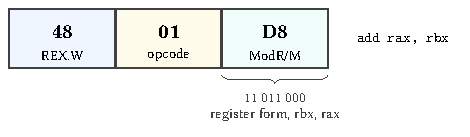
\includegraphics[width=0.72\textwidth]{figures/x64-add-encoding}
\caption{One three-byte x86-64 encoding of \code{add rax,rbx}. The byte
boundaries are regular here; the instruction family as a whole is not fixed
at three bytes.}
\figalt{Three boxes labeled 48 REX.W, 01 opcode, and D8 ModR/M, followed by add rax comma rbx.}
\label{fig:x64-add-encoding}
\end{figure}

Byte \code{48} is a REX prefix with the \(W\) bit set, selecting a 64-bit
operand size for this form. Opcode \code{01} selects ADD with a register
source and a register-or-memory destination. ModR/M byte \code{D8} is
\code{11 011 000} in binary. The \code{11} \textit{mod} field selects a
register destination rather than memory. The \code{011} \textit{reg} field
names \code{rbx}. The \code{000} \textit{r/m} field names \code{rax}.

Remove byte \code{48} and \code{01 D8} is still a valid instruction, but the
ordinary operand size is 32 bits: \code{add eax, ebx}. Changing or removing a
prefix need not make the input illegal. It can produce a nearby legal
instruction with a different state effect. That makes prefix mutations strong
negative controls.

Change ModR/M from \code{D8} to \code{18}. Its high two bits are now
\code{00}, so the destination is memory addressed through \code{rax}, not the
register \code{rax}. The decoder may then need more bytes for an addressing
form. A one-bit change has crossed from register arithmetic into a memory
operation and altered the possible failure behavior.

\begin{warning}[title={Do not infer an x86 instruction boundary from a line break}]
The next byte in a hex dump is not necessarily the next instruction. It may be
a SIB byte, displacement, or immediate belonging to the current instruction.
Conversely, a prefix-like byte may begin a separate instruction when parsing
starts at another address. Instruction boundaries come from the decoder and
the chosen starting address.
\end{warning}

This property makes a damaged byte stream especially instructive. If one
decoder consumes three bytes while another consumes two, their disagreement
does not end at the first instruction. They begin the next decode at different
addresses. A length bug can change the interpretation of the entire suffix.

\subsection{x86 decoding is a constrained walk through the bytes}

A practical x86-64 decoder cannot split every instruction into the same fixed
slots. It walks through a bounded sequence of possible components. Prefix
bytes alter mode-dependent attributes or extend fields. The opcode determines
which later components are required. A ModR/M byte can select registers or a
memory-addressing form. That form may require a SIB byte and displacement. The
selected operation may finally require an immediate.

Later choices depend on earlier ones. The same byte value can be an opcode at
one position and data for a displacement at another. A byte that resembles a
prefix has that role only while the parser is still in a prefix-accepting
position and the current mode gives it that meaning. Consequently, scanning
for familiar byte values without decoder state cannot establish boundaries.

The walk should return both a structured instance and its consumed length.
Execution uses the structured operands. The fetch loop uses the length to
calculate the following instruction address. A disassembler uses both to print
one line and advance through a buffer. If these consumers recalculate length
independently, the system contains several decoders whose disagreements can
desynchronize the program.

\begin{example}[title={A memory form expands the parse}]
In the chapter's \code{48 01 D8} example, ModR/M mode bits \code{11} finish
operand selection with registers and no displacement. Changing those bits to a
memory mode can make the remaining ModR/M fields request a SIB byte, a
displacement, or both. The opcode still belongs to ADD, but the instruction
length, operand kind, address calculation, and possible faults can all change.
\end{example}

Incomplete x86 input is therefore position-sensitive. Ending after an opcode
that requires ModR/M differs from ending inside a four-byte displacement.
Both need more bytes, but a diagnostic can name the missing component. Such
diagnostics make truncation controls much stronger than one undifferentiated
end-of-buffer error.

\begin{warning}[title={Length is part of decoder soundness}]
A decoder that selects the right operation and operands but reports the wrong
length is unsound for program execution. The current step may appear correct,
yet fallthrough begins at the wrong byte and changes the decoded suffix.
\end{warning}

\section{Three additions, three decoder shapes}

The examples perform the same broad arithmetic but do not have the same
architectural contract.

\begin{center}
\begin{tabular}{@{}p{0.19\textwidth}p{0.22\textwidth}p{0.24\textwidth}p{0.25\textwidth}@{}}
\toprule
Question & A0 & RV64I & x86-64 example\\
\midrule
Length & always four bytes & four bytes in the selected base subset & three bytes for this form\\
Operation selector & one opcode byte & opcode plus funct3 and funct7 & prefix, opcode, and ModR/M\\
Operand names & three-bit fields & five-bit fields & ModR/M fields extended by REX bits\\
Arithmetic width & parameter \(w\) & 64 bits for \code{add} & 64 bits because REX.W is set\\
Condition writes & Z, N, C, V & none & selected status flags\\
Ordinary next PC & \(pc+4\) & \(pc+4\) & \(pc+3\) for this instance\\
\bottomrule
\end{tabular}
\end{center}

The table blocks a tempting but false abstraction: ``ADD means the same thing
everywhere.'' The destination sum may correspond under a state relation, yet
the condition state, zero register, program-counter increment, legal inputs,
and failure modes differ. Cross-ISA reasoning begins by naming those
differences, not by hiding them behind a shared mnemonic.

\begin{goingdeeper}[title={A useful common decoded form}]
A comparison tool can translate all three instances into a book-owned form
such as \(
\mathrm{AddReg}(\mathit{width},dst,left,right,
\mathit{condition\ policy},\mathit{length})
\). That form is not a new universal ISA. It is an explicit bridge carrying
the facts later relations need. If the translation drops instruction length
or condition behavior, it cannot support proofs that observe those facts.
\end{goingdeeper}

\section{What decoder correctness can mean}

There is no single useful sentence called ``the decoder is correct'' until we
choose a reference and a scope. Four properties matter.

\begin{enumerate}
\item \emph{Soundness:} every accepted byte string is assigned the instruction
instance specified by the pinned source in the declared mode.
\item \emph{Completeness:} every in-scope legal encoding is accepted.
\item \emph{Length correctness:} the decoder consumes exactly the bytes
belonging to the instruction.
\item \emph{Rejection correctness:} reserved, illegal, incomplete, and
out-of-scope patterns receive the declared result rather than an invented
instruction.
\end{enumerate}

Round-trip tests help but cover narrower statements. If
\(D(E(i))=i\) for every supported instance \(i\), the encoder does not produce
an input that this decoder misreads. The property says nothing about byte
strings the encoder never emits. Conversely, if \(E(D(b))=b\) for every
accepted canonical byte string \(b\), accepted inputs reproduce their bytes.
Aliases and multiple legal encodings can require a normalization relation
instead of literal equality.

An independent decoder gives another view of the same bytes. Agreement over a
large corpus is valuable defect evidence. It is not proof against a shared
misreading of the specification, nor does it establish execution semantics.
The strongest practical route combines source-derived cases, independent
implementations, generated boundary inputs, and small proofs for regular field
operations.

\subsection{Decoder tests should cover partitions, not only examples}

Random byte strings often spend most of their time in common rejection paths.
A more informative generator partitions the input space by form, operand
boundary, reserved field, feature gate, length, and rejection class. It then
draws legal and nearby illegal cases from every partition. Coverage means that
each declared decision fired, not merely that many bytes were processed.

Mutation tests start from a source-derived legal encoding and alter one
load-bearing feature. Set each reserved bit. Move every register field across
its minimum and maximum. Change an opcode selector while holding operands
fixed. Truncate at every byte boundary. For x86, change prefix presence,
ModR/M mode, SIB demand, displacement size, and immediate length separately.
For RV64, mutate each fragment of a split immediate before checking the
reassembled value.

\begin{definition}[title={A decoder control matrix}]
A control matrix maps each decoder obligation to at least one accepted case
and one mutation expected to change its result. Rows name obligations such as
length, field extraction, reserved-bit rejection, feature selection, and
canonicality. Columns record the witness bytes, expected class, actual class,
and replay result.
\end{definition}

Differential decoding belongs in the matrix but does not replace it. When two
decoders disagree, retain the bytes, modes, versions, structured results, and
consumed lengths. Resolve the witness against the pinned primary source.
Silently choosing the majority result would turn implementation agreement into
an authority it does not possess.

The corpus should also retain boring boundary successes. A decoder that
rejects every input can pass an illegal-only suite. Legal minimum and maximum
field values, shortest and longest in-scope forms, and enabled feature cases
prove that the acceptance paths remain live.

\begin{proofkit}[title={Prove the regular pieces; test the tables}]
Field extraction is algebra. For a field of width \(k\) beginning at bit \(j\),
\[
  \mathrm{field}_{j,k}(x)=(x\mathbin{\gg}j)\mathbin{\&}(2^k-1).
\]
One can prove that packing non-overlapping bounded fields and extracting them
returns the inputs. Opcode assignments and mode-specific legality come from a
versioned table. Keep the algebraic lemma separate from the source-dependent
table check so a later manual revision does not masquerade as a change in bit
arithmetic.
\end{proofkit}

\section{The introductory Axeyum route}

Axeyum does not yet contain the architectural packages used in this chapter.
At sibling revision
\code{a9991fdad6c1e4b2bda596b46d2c8c715556ceae}, it provides reusable
bit-vector expressions, solver routes, SAT and DRAT machinery, and kernel
reconstruction infrastructure. It does not provide a reusable A0 decoder,
RV64 decoder and semantics, or x86-64 decoder and semantics. This boundary is
recorded in the book's Axeyum guide and must remain visible until code and
evidence replace the implementation obligations.

The first Axeyum exercise is therefore constructive. Define a small A0 decoded
instruction type. Write a total decoder returning either a legal instance or
a named rejection. Add an encoder for legal instances. Prove or exhaustively
check the round trip at a small word width, then run controls that set every
reserved or unused field.

The next layer can reuse Axeyum's word machinery to express field extraction
and packing. A solver can search for a byte string that passes the decoder but
fails re-encoding, or two legal instances that encode to the same bytes. A SAT
or SMT result is a search result. Promotion to book evidence still requires a
manifest, exact source revision, replay route, and negative control.

For RV64I and x86-64, do not begin by implementing the whole architecture.
Pin the manual, select the chapter's finite instruction forms, record the
mode and feature set, and build a decoder whose public result includes length.
Compare against an independent mature decoder, but keep the book-owned rule as
the object under test. Execution semantics come afterward.

\begin{sidebar}[title={Four questions to ask of every decoder run}]
Which exact manual revision supplies the rule? Which mode and extensions are
enabled? How many bytes did the decoder consume? What changed when a reserved
bit, prefix, field, or final byte was mutated? A transcript without those
answers is difficult to interpret and too weak for a load-bearing claim.
\end{sidebar}

\section{Where the model stops}

This chapter does not define all RV64I or x86-64 encodings. It does not cover
RISC-V compressed instructions, vectors, privilege, or every extension. It
does not cover the full x86 prefix history, VEX, EVEX, APX, every addressing
form, or the maximum instruction length. Later chapters add selected forms
only when a proof needs them.

It also does not claim that equal decoded arithmetic establishes equal program
behavior. The next chapters add data movement, address formation, arithmetic
conditions, control transfer, and calling conventions. Only after those
effects are explicit can Parts III and IV define equivalence and refinement
between machines.

The working discipline is now fixed: preserve the original bytes, state the
mode and enabled features, return length explicitly, distinguish every
rejection class, and connect execution only to a legal structured instance.
That discipline scales from A0's four transparent bytes to a variable-length
x86 stream without pretending their decoder problems are identical.

\section{Exercises}

\begin{enumerate}
\item \textbf{Execute.} Decode \code{10 2B 02 00} under A0. List every
legality check, the structured result, the number of bytes consumed, and the
next program counter after execution.

\item \textbf{Break.} Construct four mutations of that A0 encoding: wrong
opcode, reserved bit, unused condition, and nonzero immediate. State the
required rejection for each.

\item \textbf{Prove.} Prove that packing and extracting A0's \(rd\) and
\(rs1\) fields round trips for register numbers below eight. Identify exactly
where the range premise is used.

\item Pack RV64I \code{sub x3,x5,x2}. Give the 32-bit word and its four
little-endian memory bytes. Explain which one field differs from the addition
example.

\item Starting from RV64I word \code{002281B3}, change only \(rd\) to zero.
Separate what changes in the decoded instance from what changes in execution.

\item Decode x86-64 bytes \code{48 01 D8} by naming the contribution of every
byte. Then remove \code{48}; explain why the remaining sequence is not merely
an incomplete version of the same instruction.

\item Change ModR/M \code{D8} to \code{18}. Which field changed, and why can
the new form involve memory and additional addressing bytes?

\item Give an example showing why \(D(E(i))=i\) does not establish that the
decoder rejects all illegal byte strings.

\item \textbf{Transfer.} Design a common decoded addition object rich enough
to represent the three chapter examples. Mark which fields belong to decoding
and which belong only to execution.

\item Design a differential test manifest for one RV64I form or one x86-64
form. Include the source pin, mode, generator domain, independent decoder,
expected agreement, and at least two negative controls.
\end{enumerate}
